\documentclass[10pt]{article}
\usepackage[utf8]{inputenc}\usepackage[T1]{fontenc}\usepackage[letterpaper,margin=1.55cm]{geometry}
\usepackage{graphicx,booktabs,xcolor,amsmath,hyperref,array}\definecolor{navy}{HTML}{102A43}\definecolor{teal}{HTML}{2A9D8F}
\hypersetup{colorlinks=true,urlcolor=teal}\setlength{\parindent}{0pt}\setlength{\parskip}{5pt}
\begin{document}\begin{titlepage}\pagecolor{navy}\color{white}\raggedright\vspace*{1cm}{\Large DEEP LEARNING Y SISTEMAS INTELIGENTES\par}\vspace{1cm}{\Huge\bfseries Proyecto 1\\Monitoreo transaccional --- V4\par}\vspace{.7cm}{\LARGE Ingeniería causal, expertos y validación temporal\par}\vfill{\Large Universidad del Valle de Guatemala\\Kevin Recinos · Grupo 1 · Sección 30\\Semestre II 2026\par}\vspace{1cm}{\Large Wilson Alejandro Calderón Argueta · 22018\\Pablo Daniel Barillas Moreno · 22193\par}\vfill\textbf{Estado:} candidato congelado post-hoc; V3 permanece confirmada hasta una cohorte nueva.\end{titlepage}\nopagecolor

\section*{Resumen ejecutivo} Se analizaron 590,540 transacciones IEEE-CIS con prevalencia 3.50\%. V4 integra 569 columnas tras ingeniería y selecciona 360 numéricas más 38 categóricas. LightGBM optimizado alcanza AP walk-forward 0.6175 y ROC-AUC media 0.9220. El candidato experto por ProductCD, seleccionado antes de calibración y evaluación, obtiene AP 0.5491, ROC-AUC 0.9012, precisión 0.2024, recall 0.7652, F1 0.3201 y costo Q605,520. Mejora todas las métricas frente a V3, pero la política recall $\ge0.75$ es post-hoc; requiere cohorte nueva.

\section{Problema y datos} El fraude representa 3.50\%; accuracy convencional sería engañosa. Se priorizan AUC-PR, precisión, recall, F1, costo y top-K. Las tablas se unen con TransactionID y ordenan con TransactionDT; ninguno entra como magnitud predictiva. Para cada transacción, $x_t^{hist}=f(\{x_j:t_j<t\})$. Se utiliza 70\% train, 15\% validación y 15\% benchmark histórico reutilizado.

\section{Ingeniería causal} V4 añade calendario, forma del monto, resúmenes V/C/D, $D_i-día$, $\log(1+C_i)$, ausencias, frecuencias previas, cambios de contexto y estadísticas para tarjeta--dirección, tarjeta--correo, tarjeta--dispositivo y tarjeta--producto. IDs no se usan como números continuos. Selección y correlación se aprenden en el 55\% inicial; solo se podan sustitutos con $|\rho_s|\ge0.999$. PCA no se aplica al boosting porque en V3 perdió AP aun conservando 99.53\% de varianza.
\newpage
\section{Modelos y protocolo} Optuna ejecuta 18 pruebas sobre hojas, profundidad, regularización, submuestreo y suavizado categórico. Se comparan LightGBM, XGBoost y CatBoost piloto, hard-negative mining, expertos W/NO-W y stacking. CatBoost y XGBoost usan 120/220 iteraciones por costo de CPU; son ablations, no búsquedas exhaustivas. La validación se divide para early stopping, meta, selección de candidato, calibración, umbral y evaluación.

\begin{figure}[h]\centering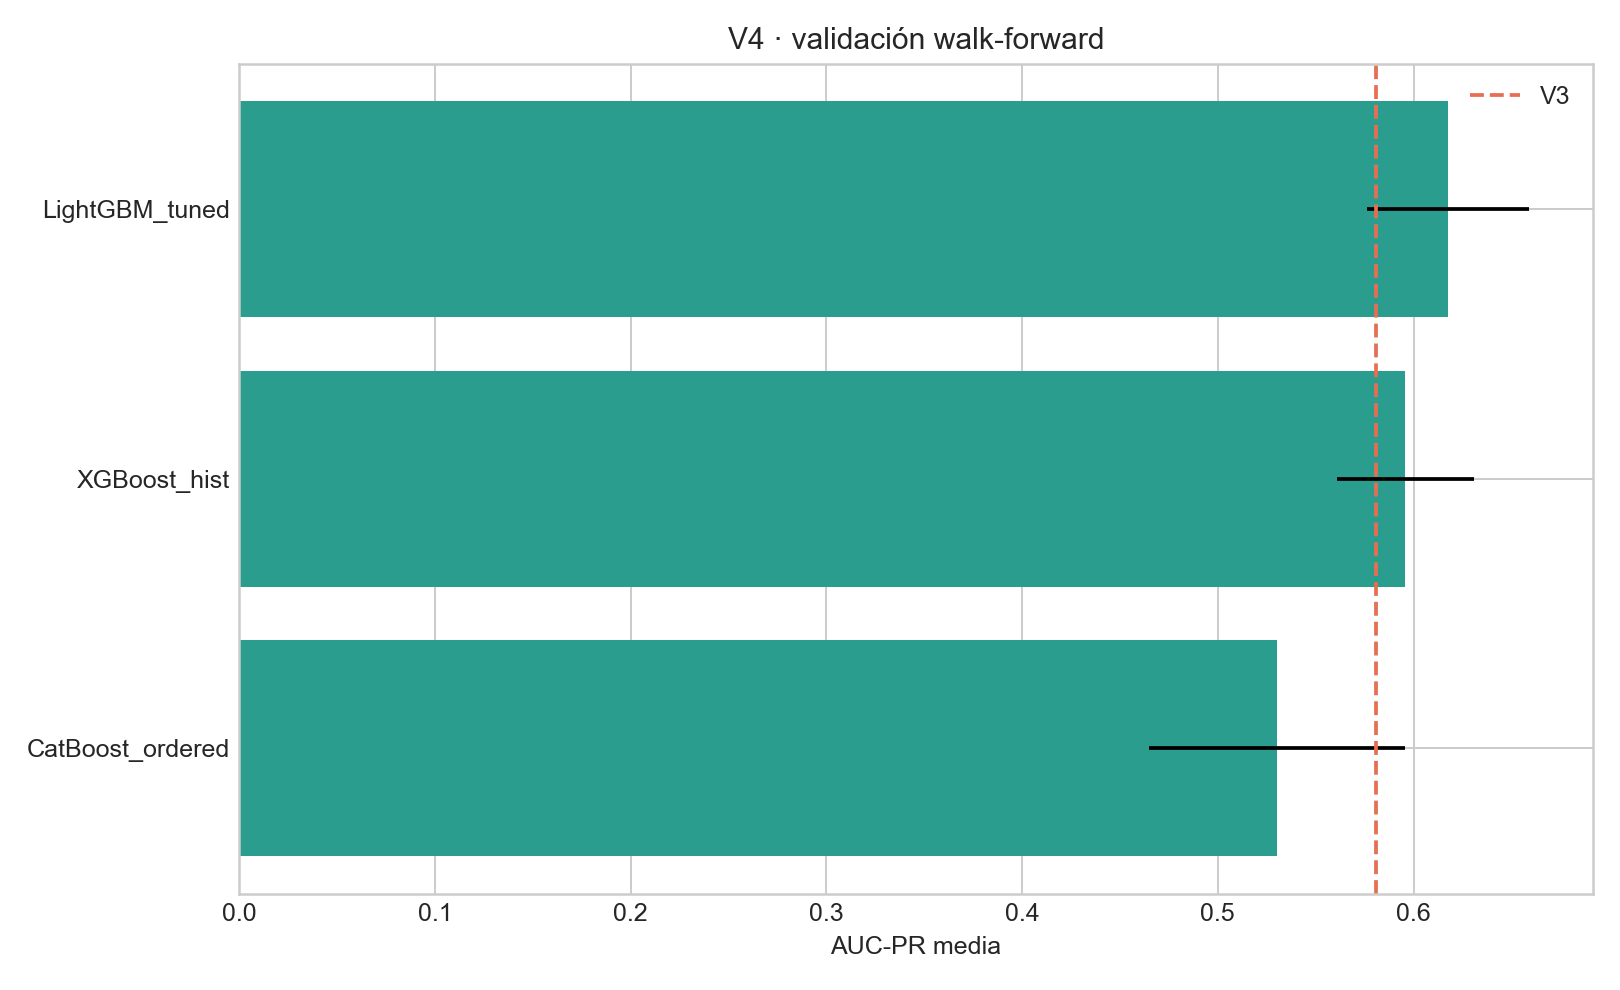
\includegraphics[width=.78\linewidth]{../../../evidencia/figuras/v4/01_walk_forward_v4.png}\caption{AUC-PR walk-forward de candidatos V4.}\end{figure}

LightGBM obtiene AP media 0.6175 (DE 0.0412), mejora V3 en 0.0366 y supera 0.90 de ROC-AUC media. XGBoost obtiene 0.5957 y CatBoost piloto 0.5302. La ventaja de LightGBM aumenta cerca del período final.
\newpage
\section{Selección y resultados} El bloque 50--60\% de validación selecciona el candidato antes de calibración y umbral. Expertos ProductCD ganan con AP 0.6078; stacking obtiene 0.6007, pero reduce ROC-AUC de evaluación a 0.8686 y se descarta.

\begin{center}\begin{tabular}{lrrrrrr}\toprule Modelo&AUC-PR&ROC-AUC&Prec.&Recall&F1&Costo\\\midrule V3&0.445&0.890&0.163&0.710&0.265&Q743,280\\\textbf{V4}&\textbf{0.549}&\textbf{0.901}&\textbf{0.202}&\textbf{0.765}&\textbf{0.320}&\textbf{Q605,520}\\\bottomrule\end{tabular}\end{center}

V4 aumenta AP 0.1041, ROC-AUC 0.0112, precisión 0.0397, recall 0.0556 y F1 0.0554; reduce costo 18.5\%. La diferencia pareada AP es 0.1041, IC 95\% [0.0696, 0.1426].

\begin{figure}[h]\centering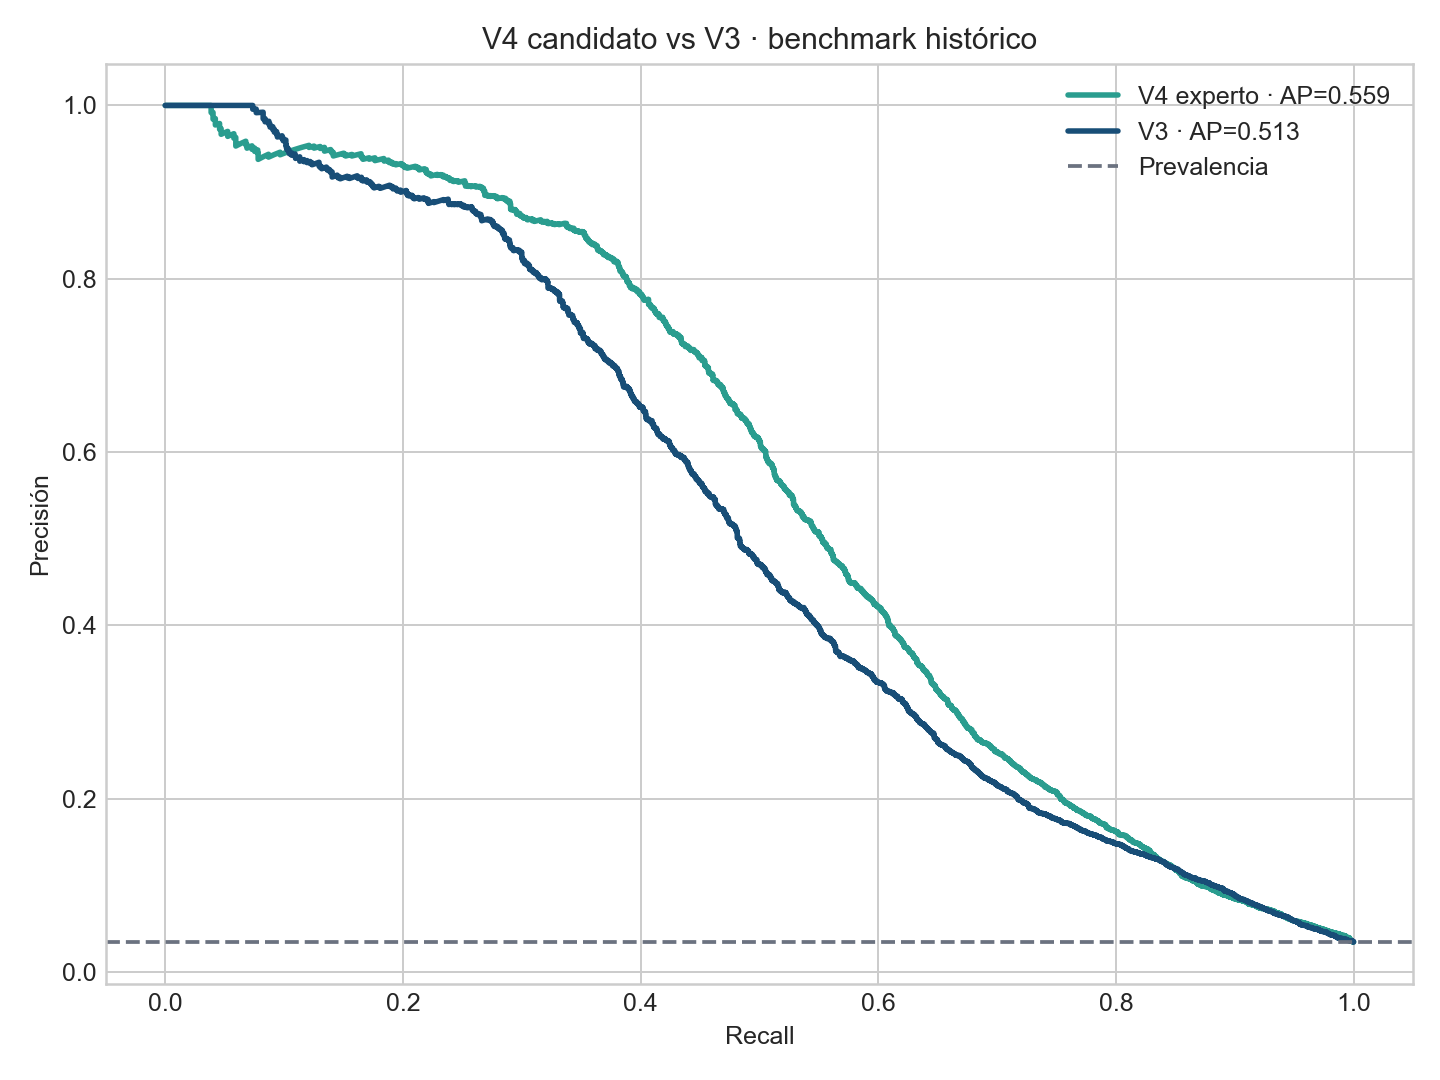
\includegraphics[width=.70\linewidth]{../../../evidencia/figuras/v4/07_curvas_pr_candidato_v4.png}\caption{Curvas PR V3/V4 en benchmark histórico reutilizado.}\end{figure}
\newpage
\section{Calibración, umbral y capacidad} La calibración del candidato reduce Brier de 0.0245 a 0.0237 y ECE de 0.0156 a 0.0060. El umbral robusto 0.05664 exige recall 0.75 en selección para amortiguar deriva y el costo FN/FP de 23.3:1.

La política balanceada prioriza F1; la económica eleva recall a 0.813, pero baja precisión. En el benchmark V4 obtiene AP 0.5592, ROC-AUC 0.9013, precisión 0.2152, recall 0.7399 y costo Q4,866,000. Al revisar 1\% de mayor riesgo, precision@K supera 0.90 y recall@K ronda 0.26.

\begin{figure}[h]\centering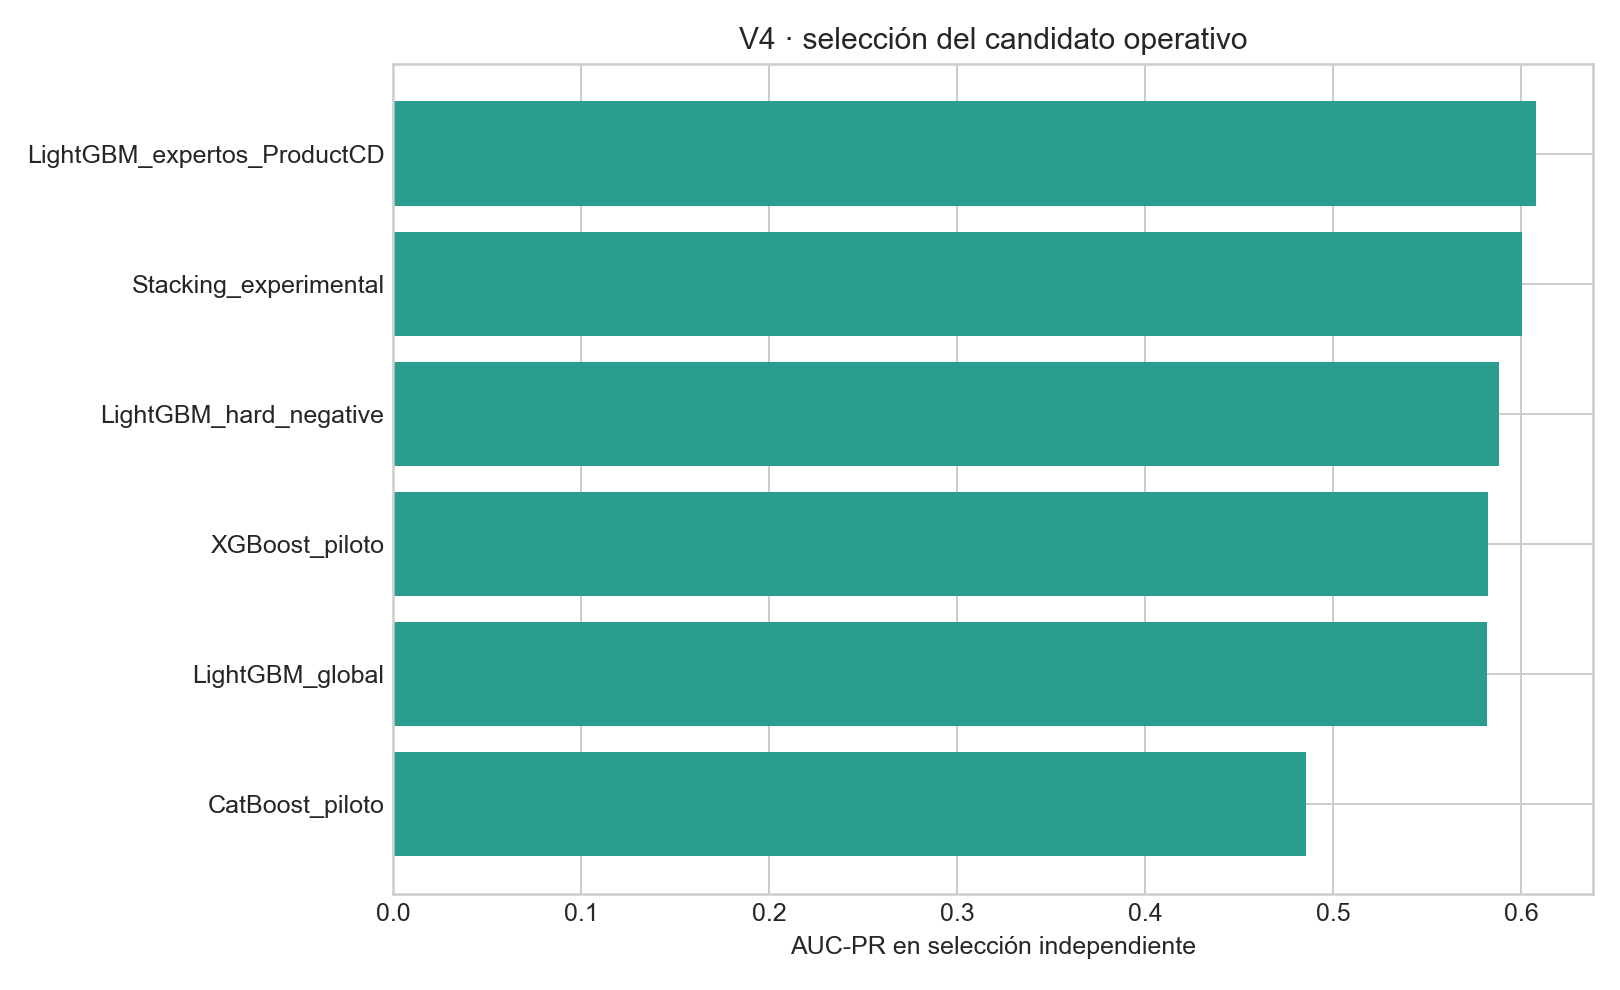
\includegraphics[width=.68\linewidth]{../../../evidencia/figuras/v4/06_seleccion_candidato_v4.png}\caption{Selección del candidato en bloque independiente.}\end{figure}
\newpage
\section{Deriva, limitaciones y decisión} La validación adversarial alcanza ROC-AUC 1.0, dominada por day\_index y acumulados; demuestra separación temporal y justifica walk-forward, no perfección del fraude. Deben separarse deriva total y residual sin tiempo explícito en una cohorte futura.

Limitaciones: benchmark reutilizado, identidad proxy, datos anonimizados, costos académicos, presupuesto piloto CatBoost/XGBoost y ausencia de cohorte externa. V4 no debe bloquear transacciones ni atribuir culpabilidad; prioriza revisión humana. Antes de producción se requieren privacidad, seguridad, explicabilidad, sesgos, costos reales, latencia, monitoreo y apelación.

\textbf{Decisión:} V4 domina V3 bajo la política robusta, pero esa política fue añadida después de observar la primera evaluación. Se congela el pipeline, las 398 variables, los modelos, calibrador y umbral; V3 permanece confirmada hasta evaluar V4 una sola vez y sin ajustes en una cohorte temporal nueva.

\section*{Referencias}\small Akiba, T., et al. (2019). Optuna. \textit{KDD}, 2623--2631.\\Chen, T., \& Guestrin, C. (2016). XGBoost. \textit{KDD}, 785--794.\\IEEE CIS. (2019). \textit{IEEE-CIS Fraud Detection}. Kaggle.\\Ke, G., et al. (2017). LightGBM. \textit{NeurIPS, 30}.\\Prokhorenkova, L., et al. (2018). CatBoost. \textit{NeurIPS, 31}.\\Saito, T., \& Rehmsmeier, M. (2015). Precision-recall plots for imbalanced data. \textit{PLOS ONE, 10}(3).

\section*{Declaración de IA} IA apoyó código, redacción, visualización y auditoría. Los autores ejecutaron, verificaron y asumen responsabilidad.\end{document}